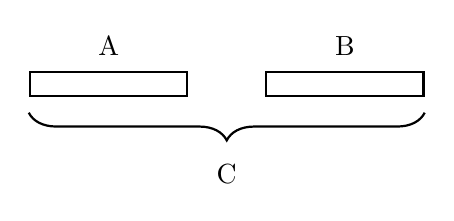
\begin{tikzpicture}

    % Define the two rectangles
    \node[draw, rectangle, minimum width=2cm, minimum height=0.3cm, thick] (boxA) at (0,0) {};
    \node[draw, rectangle, minimum width=2cm, minimum height=0.3cm, thick] (boxB) at (3,0) {};

    % Add labels A and B above the rectangles
    \node at (boxA.north) [above=2pt] {A};
    \node at (boxB.north) [above=2pt] {B};

    % Draw the brace spanning from the bottom-left of A to the bottom-right of B
    % 'mirror' puts the brace below the line
    \draw [decorate, decoration={brace, amplitude=10pt, mirror}, thick] 
        ([yshift=-0.2cm]boxA.south west) -- ([yshift=-0.2cm]boxB.south east) 
        node[midway, below=15pt] {C};

\end{tikzpicture}
